\subsection*{Checkpoint 1.18: Evaluating Trigonometric Functions}

\subsubsection*{Instruction}

\begin{enumerate}[label=(\alph*)]
  \item
    Evaluate $ cos(3\pi/4) $.
  \item
    Evaluate $ sin(-\pi/6) $.
\end{enumerate}

\subsubsection*{Solution}

\begin{enumerate}[label=(\alph*)]
  \item
    We start by sketching an unit circle with the angle $ 3\pi/4 $, see figure \ref{figure:checkpoint-1.1.18-a}. We know that $ cos(3\pi/4) $ is defined to be the $ x $-coordinate of the point sketched on the unit circle.

    \begin{figure}
      \centering
      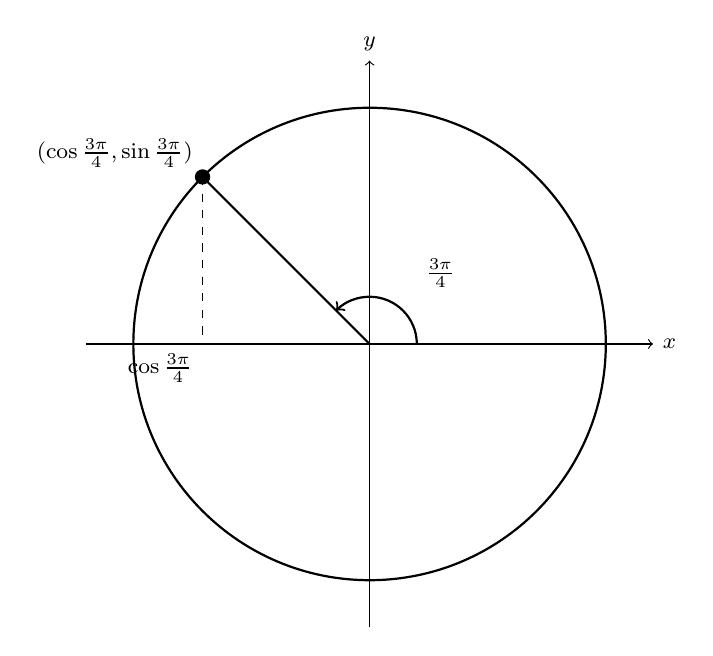
\begin{tikzpicture}[scale=3]
        % Draw the unit circle
        \draw[thick] (0,0) circle(1);

        % Axes
        \draw[->] (-1.2,0) -- (1.2,0) node[right] {\footnotesize $x$};
        \draw[->] (0,-1.2) -- (0,1.2) node[above] {\footnotesize $y$};

        % Angle 3π/4 (135 degrees)
        \draw[thick] (0,0) -- (-0.7071,0.7071);
        \filldraw (-0.7071,0.7071) circle(0.03) node[above left] {\footnotesize $(\cos \frac{3\pi}{4}, \sin \frac{3\pi}{4})$};

        % Draw the cosine value as a horizontal projection
        \draw[dashed] (-0.7071,0.7071) -- (-0.7071,0) node[below left] {\footnotesize $\cos \frac{3\pi}{4}$};

        % Mark the angle
        \draw[thick,->] (0.2,0) arc[start angle=0,end angle=135,radius=0.2];
        \node at (0.3,0.3) {\footnotesize $\frac{3\pi}{4}$};
      \end{tikzpicture}
      \caption{Unit circle with point at angle $ 3\pi/4 $}
      \label{figure:checkpoint-1.1.18-a}
    \end{figure}

    We can see a right triangle in the picture. We know that this triangle will have equal base and height, due to that our angle splits fourth quadrant exactly in half. We also know that the hypotenuse is $ 1 $, because of the unit circle with radius $ 1 $. The Pythagorean theorem gives us $ 1^2 = \sqrt{x^2 + x^2} $, which after some calculations leads us to that $ x = \pm\sqrt{2}/2 $. We can see from the figure that $ x $ will be negative which leads to that $ cos(3\pi/4) = -\sqrt{2}/2 $
  \item
    TODO
\end{enumerate}

\subsubsection*{Answer}

\begin{enumerate}[label=(\alph*)]
  \item
    $ cos(3\pi/4) = -\sqrt{2}/2 $.
  \item
    TODO
\end{enumerate}
